\documentclass[11pt]{article}
\usepackage{fullpage}
\usepackage{graphicx}
\usepackage{url}
\usepackage{float}
\usepackage{amsmath}

\title{CS140 - Assignment 3\\\small{Due: Sunday,  Feb. 11 at 10pm}}
\author{}
\date{}


\begin{document}
\maketitle

\begin{center}
% \includegraphics[scale=0.6]{figures/entomology.jpg}

\footnotesize{http://www.xkcd.com/1012/}
\end{center}

\noindent You must work with a partner on this assignment, but it can be anyone in the class, including someone that you've previously worked with.  If you need a partner, please reach out ASAP.

\begin{enumerate}

\item \textbf{[25 points]} Stock Market Problem - the code

Implement your algorithm from the previous assignment for the stock market problem in Python, C, or
  Java (ask me first if you want to use another language).
  
  Your submissions should be called \texttt{stockmarket.c}, \texttt{stockmarket.py}, or \texttt{StockMarket.java} if you're using C, Python, or Java, respectively.  We will use an autograder that relies on this naming convention.
  
  Your code must allow the user to specify two filenames on the command line, say {\tt
    infile.txt} and {\tt outfile.txt} (these could be any filename, but I'm using these for examples.)  We don't
  want to edit your code, so they need to be command-line parameters.  For example:
  \begin{itemize}
  \item If using C, your code might be compiled and executed as follows:
\begin{verbatim}
  % gcc stockmarket.c -o stockmarket
  % ./stockmarket infile.txt outfile.txt
\end{verbatim}
\item If using Python 3\footnote{See the
  \url{https://docs.python.org/3/howto/argparse.html} module.}, your
  code might be executed as follows:
\begin{verbatim}
  % python3 stockmarket.py infile.txt outfile.txt
\end{verbatim}
\item If using Java\footnote{See \url{https://docs.oracle.com/javase/tutorial/essential/environment/cmdLineArgs.html}}, your code might be compiled and
  executed as follows:
\begin{verbatim}
  % javac StockMarket.java
  % java StockMarket infile.txt outfile.txt
\end{verbatim}
  \end{itemize}
    
  The contents of the input file will be in the
  following form:
  \begin{verbatim}
    8
    42
    40
    45
    45
    44
    43
    50
    49
\end{verbatim}
The first line specifies the number of days (which may not always be a power of 2).  The
following lines give the value of the stock on each day.  

In this case the output file should contain the following:
\begin{verbatim}
    3
    2
    40
    45
    45
\end{verbatim}
The first line gives the length of the longest non-decreasing subsequence,
the second line gives the day on which the subsequence begins (note the
1-based indexing!), and the rest of the lines give the prices of the
stock on the days included in the subsequence.  If there is more than one
longest non-decreasimg subsequence, your code can return either one.

Most of the grade for this problem will be based on correctly implementing a
divide-and-conquer algorithm that solves the problem described in
last week's assignment.  Note that we will evaluate outputs using
{\tt diff} so please make sure your output 
is in the format described above!  We may also
consider code efficiency in an absolute (wall clock) sense.  

(Small) sample input and output files are on the course webpage.


\item \textbf{[25 points]} More Fun with Binary Search Trees
 
\begin{enumerate}

\item \textbf{[5 points]} Is the operation of deletion ``commutative'' in that deleting $x$ and then $y$ from a binary search tree always leaves the same tree as deleting $y$ and then $x$? Argue why it is or give a counterexample.  \textit{Hint:} There are three different cases for deleting in a binary tree.  Make sure you think about all of them. (We'll use the algorithm discussed in class, i.e., if a node has two children, it is replaced with its successor.)

\textbf{Answer}: No. 

A counter-example: consider this example binary search tree:
\begin{figure}[H]
  \centering
  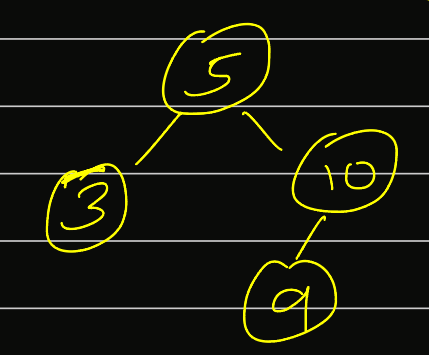
\includegraphics{IMG_3438.png}
  \caption{Example BST}
  \label{fig:yourlabel}
\end{figure}

Let $x=5$ and $y=3$.

Consider case I where we delete x first, then y.
\begin{figure}[H]
  \centering
  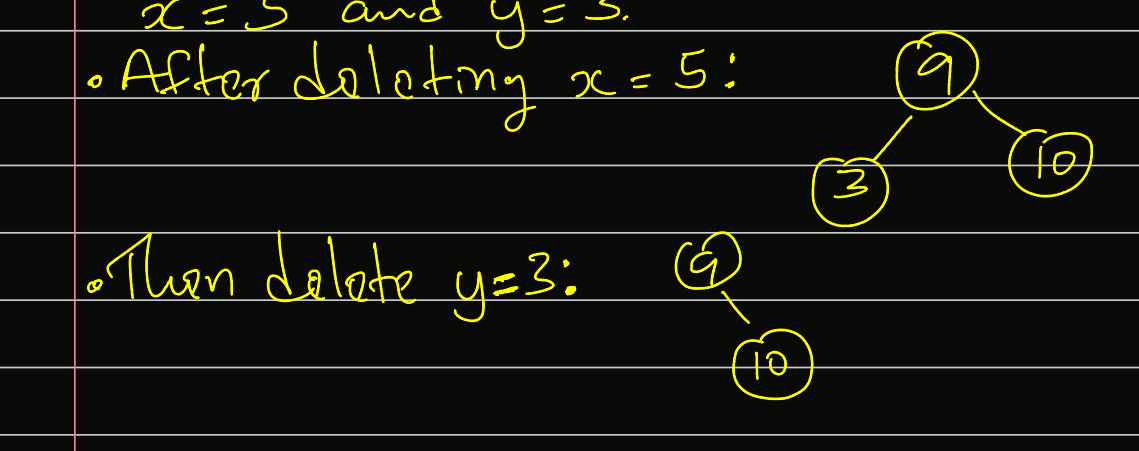
\includegraphics[width=\textwidth]{IMG_5015.png}
  \caption{Deleting x then y}
  \label{fig:yourlabel}
\end{figure}

Consider case II where we delete y first, then x.
\begin{figure}[H]
  \centering
  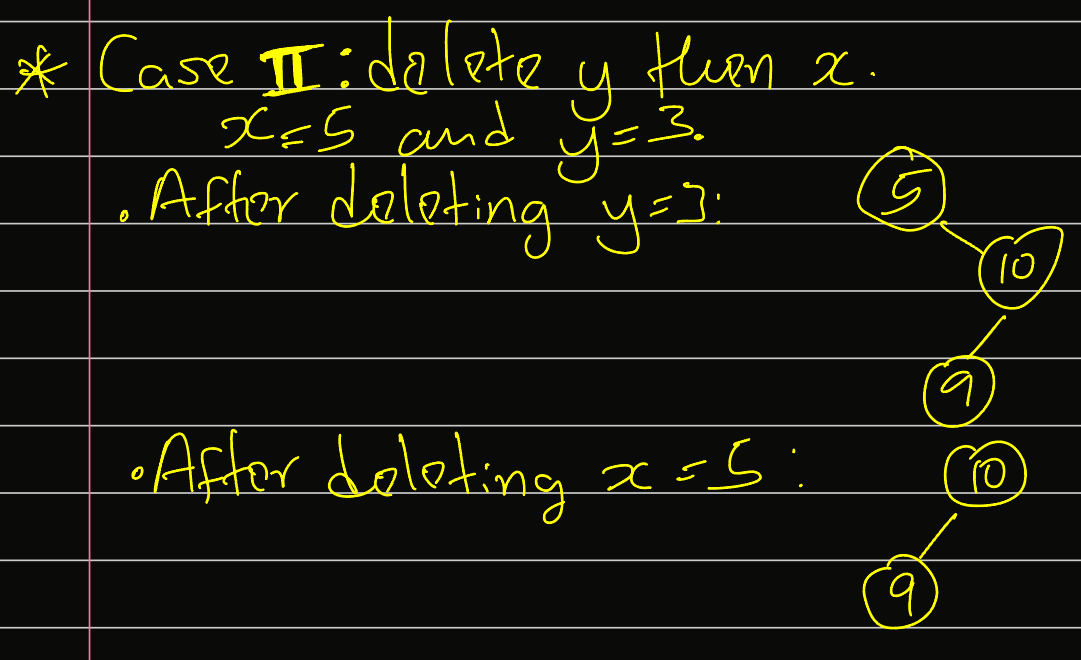
\includegraphics[width=\textwidth]{IMG_2743.png}
  \caption{Deleting y then x}
  \label{fig:yourlabel}
\end{figure}

We can therefore conclude that:
\begin{figure}[H]
  \centering
  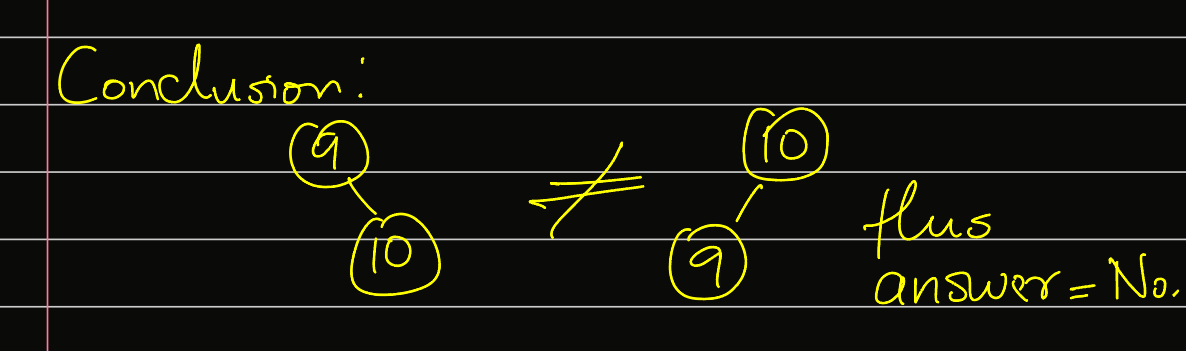
\includegraphics[width=\textwidth]{IMG_3706.png}
  \caption{Conclusion: Commutation of deletion does not apply to BSTs}
  \label{fig:yourlabel}
\end{figure}

\item \textbf{[20 points]} Balanced? 

Red-black trees maintain a set of five properties; in class we showed
that maintaining those properties guarantees that the height of a
red-black tree with $n$ nodes is never more than $2\log(n+1)$.
Consider another balanced binary search tree which maintains the
following invariant: for any node $x$, the heights of the left and
right subtrees of $x$ differ by at most $1$.  We'll call these 1off
trees.

\begin{enumerate}
\item {[14 points]} Prove by strong induction on the height of the tree that a 1off
  tree with height $h$ has at least $f(h)$ nodes, where $f(h)$ is the
  $h$th Fibonacci number.  (Recall that $f(n) = f(n-1)+f(n-2)$ and
  that $f(0) = f(1) = 1$.)

\textbf{Answer}:

\emph{Claim}: For a 1off tree of height $h$, the minimum number of nodes present is at least $f(h)$, where $f(h)$ denotes the $h$-th Fibonacci number.

\emph{Base Cases}: The Fibonacci sequence initiates with $f(0) = f(1) = 1$. Our proof should thus involve two foundational scenarios:

- \textbf{Base Case 1}: For a solitary leaf node, where $h=0$, the Fibonacci sequence yields $f(0) = 1$. This is consistent, as a single-node tree (or a leaf) inherently possesses a height of 0, aligning the Fibonacci count with the tree's node count.

- \textbf{Base Case 2}: For a tree comprising a root and a single child, denoted by $h=1$, the Fibonacci sequence similarly provides $f(1) = 1$. Although the tree encompasses two nodes, the stipulation necessitates at least $f(h) = f(1) = 1$ node, affirming the claim for this second base case.

\emph{Inductive Step}: Adopting strong induction, let us presume that the claim holds true for all heights up to $h$—that is, a 1off tree of height $h$ encompasses at least $f(h)$ nodes, as our inductive hypothesis.

To extend this claim to a tree of height $h+1$, consider the structure of such a tree, inclusive of its left and right subtrees, without delving into the specifics of node values. The inductive hypothesis suggests that:

- The left subtree, at height $h$, contains no fewer than $f(h)$ nodes.

- The right subtree, maintaining a height of either $h$ or $h-1$, adheres to the hypothesis, involving at least $f(h-1)$ nodes for the latter scenario.

The aggregate node count for the tree thus becomes $1 + f(h) + f(h-1)$, paralleling the Fibonacci sequence's principle that $f(h+1) = f(h) + f(h-1)$. This deduction substantiates our initial claim through strong induction, demonstrating that a tree of height $h+1$ indeed harbors a minimum of $f(h+1)$ nodes.

\item {[3 points]} Use the previous part to show that a 1off tree with height $h$ has
  at least $2f(h-2)$ nodes.
  
\textbf{Answer}:

Given the recurrence relation inherent to the Fibonacci sequence, $f(h) = f(h-1) + f(h-2)$, we observe the following for $h > 1$: the term $f(h-1)$ strictly exceeds $f(h-2)$.

This observation leads to the conclusion that $f(h) = f(h-1) + f(h-2) \ge 2f(h-2)$. Hence, we can deduce that a 1off tree with height $h$ encompasses at least twice as many nodes as a tree of height $h-2$.

\item {[3 points]} Finally show that a 1off tree with $n$ nodes has $O(\log n)$ height.

\textbf{Answer}:

In the preceding question, we established that $f(h) > 2 \cdot f(h-2)$. By setting $h' = h - 2$, we deduce that $f(h-2) \geq 2 \cdot f(h-4)$. Integrating this with our previous result, $f(h) > 2 \cdot f(h-2)$, yields $f(h) \geq 2^2 \cdot f(h-4)$. Following this reasoning further, we infer $f(h) \geq 2^3 \cdot f(h-6)$, and the pattern continues.

This iterative process allows us to generalize the relationship as: $f(h) \geq 2^j \cdot f(h - 2j)$. We can determine what $j$ is when we hit the base case and then we can continue.

\emph{Base Case}: For a tree with only a leaf, its height is zero by definition, hence $h - 2j = 0$. Consequently, we find $h = 2j$ and therefore $j = \frac{h}{2}$.

Given the established inequality $f(h) \geq 2^j \cdot f(h - 2j)$, and applying the base case, we derive $f(h) \geq 2^{\frac{h}{2}}$.

To examine the height \(h\) of a 1off tree with \(n\) nodes and ascertain if it has \(O(\log n)\) height, we manipulate the inequality with logarithmic properties: $\log(f(h)) \geq \frac{h}{2} \cdot \log(2)$, simplifying to $2 \cdot \log(f(h)) \geq h \cdot \log(2)$. This leads us to $h \cdot \log(2) \leq 2 \cdot \log(f(h))$, and hence $h \leq 2 \cdot \log\left(\frac{f(h)}{2}\right)$.

Thus, we demonstrate that the height \(h\) is indeed of the order \(O(\log n)\).
\end{enumerate}

\end{enumerate}


\subsection*{Submitting}

On Gradescope, you'll see two separate entries for this assignment (Assignment 3.1 for problem 1 and Assignment 3.2 for problem 2).  For problem 1, submit your code as a single file with the appropriate extension.  For problem 2, your answer should be a pdf, like you usually submit.


\end{enumerate}
\end{document}
